\begin{center}
	\zihao{4}\heiti
	% 中国科学院大学\\
	\LARGE{$\boldsymbol{2006}$年硕士学位研究生入学统一考试试题\\
	电动力学B卷}

\end{center}
\noindent
考生须知：\\
1.本试卷满分为150分,全部考试时间总计180分钟。\\
2.所有答案必须写在答题纸上,写在试题纸上或草稿纸上一律无效。

\vspace*{2ex}
\hrule
\vspace*{4ex}

\fancypagestyle{mypagestyle}{%
	\fancyhf{}% Clear header/footer
	\fancyfoot[OR]{第~\thepage~页，共~\pageref{LastPage}~页}%
	\fancyfoot[EL]{第~\thepage~页，共~\pageref{LastPage}~页}%
	\fancyfoot[OL]{科目名称：电动力学 }%
	\fancyfoot[ER]{科目名称：电动力学 }%
	\renewcommand{\headrulewidth}{0pt}% Header rule of .4pt
	\renewcommand{\footrulewidth}{0.5pt}% Header rule of .4pt
}
\fancypagestyle{plain}{%
	\fancyhf{}% Clear header/footer
	\fancyfoot[OR]{第~\thepage~页，共~\pageref{LastPage}~页}%
	\fancyfoot[EL]{第~\thepage~页，共~\pageref{LastPage}~页}%
	\fancyfoot[OL]{科目名称：电动力学 }%
	\fancyfoot[ER]{科目名称：电动力学 }%
}

\setcounter{page}{1}%设置页面计数器
\pagestyle{mypagestyle}

\onehalfspacing
% 排版结束，下面是题目
\vspace{0.8cm}

\noindent
一、\hspace{0.2em}问答题（共25分，请写在答题纸上）

\noindent
1.\hspace{0.8em}试用相对论形式写出麦克斯韦方程组。

\noindent
2.\hspace{0.8em}写出四维波矢量$\boldsymbol{k_{\mu}}$的四个分量。

\noindent
3.\hspace{0.8em}四维体积元$\large{\boldsymbol{d^4x=dx_1dx_2dx_3dx_4}}$是相对量还是不变量？为什么？

\vspace{0.5cm}
\noindent
二、\hspace{0.2em}选择题（共7题，每题5分，每一小题要求选取一个正确答案，请写在答题纸上）

\noindent
1.\hspace{0.8em}如果一个矩形空腔波导管内填满了相对介电常数为$\large{\boldsymbol{\varepsilon_r}}$的电介质，那么其截止频率$\large{\boldsymbol{f_d}}$与原没有填充介质的空腔的截止频率$\large{\boldsymbol{f_0}}$之间的关系为：（角标d和0分别表示电介质和真空）

\vspace{0.4cm}
(a)\hspace{0.6em}$\large{{f_d} = \boldsymbol{\varepsilon_r} {f_0}}$\hspace{1.6em}(b)\hspace{0.6em}$\large{{f_d} = \displaystyle{\frac{1}{\boldsymbol{\varepsilon_r}}} {f_0}}$\hspace{1.6em}(c)\hspace{0.6em}$\large{{f_d} = \sqrt{\boldsymbol{\varepsilon_r}} {f_0}}$\hspace{1.6em}(d)\hspace{0.6em}$\large{{f_d} = \displaystyle{\frac{1}{\sqrt{\boldsymbol{\varepsilon_r}}}} {f_0}}$
\vspace{0.4cm}

\noindent
2.\hspace{0.8em}一光源在其静止的参考系中辐射的频率为$\large{\boldsymbol{\omega_0}}$，则以速度$v$向该光源运动的观察者记录到的频率$\large{\boldsymbol{\omega}}$为

\vspace{0.4cm}
(a)\hspace{0.6em}$\large{\boldsymbol{\omega}}$ = $\large{\boldsymbol{\omega_0}} \sqrt{1- \large{\boldsymbol{\beta^2}}}$\hspace{1.0em}(b)\hspace{0.6em}$\large{\boldsymbol{\omega}} $ = $\displaystyle{\large{\boldsymbol{\omega_0}} \sqrt{1- \large{\boldsymbol{\beta}}}}$\hspace{1.0em}(c)\hspace{0.6em}$\large{\boldsymbol{\omega}}$ = $\displaystyle{\large{\boldsymbol{\omega_0}} \sqrt{ \large{\boldsymbol{\frac{1-\beta}{1+\beta}}}}}$\hspace{1.0em}(d)\hspace{0.6em}$\large{\boldsymbol{\omega}}$ = $\displaystyle{\large{\boldsymbol{\omega_0}} \sqrt{ \large{\boldsymbol{\frac{1+\beta}{1-\beta}}}}}$
\vspace{0.4cm}

\noindent
3.\hspace{0.8em}光在两种介质分界面垂直入射时，反射系数R等于：

\vspace{0.4cm}
(a)\hspace{0.6em}$\displaystyle{\large{  {(\frac{1}{n+1})}^2 }}$\hspace{1.6em}(b)\hspace{0.6em}$\displaystyle{\large{  {(\frac{1}{n-1})}^2 }}$\hspace{1.6em}(c)\hspace{0.6em}$\displaystyle{\large{  {(\frac{n-1}{n+1})}^2 }}$\hspace{1.6em}(d)\hspace{0.6em}$\displaystyle{\large{  {(\frac{n+1}{n-1})}^2 }}$
\vspace{0.4cm}

\noindent
4.\hspace{0.8em}在两个夹角为$\ang{45}$的接地导体平板之间有一点电荷q，用电相法求解此区间的电场时，其象电荷的数目为：

\vspace{0.3cm}
(a)\hspace{0.6em} 四个 \hspace{1.6em}(b)\hspace{0.6em} 五个\hspace{1.6em}(c)\hspace{0.6em} 六个 \hspace{1.6em}(d)\hspace{0.6em} 七个
\vspace{0.3cm}

\noindent
5.\hspace{0.8em}真空中一束自然光线的磁场可以准确的描述为：

\vspace{0.3cm}
(a)\hspace{0.6em}同时平行于电场和光传播方向 \hspace{4.2em}(b)\hspace{0.6em}同时垂直于电场和光传播方向\hspace{1.6em}

(c)\hspace{0.6em}与电场垂直，并且平行于光传播方向\hspace{1.6em}(d)\hspace{0.6em}与电场平行，并且垂直于光传播方向
\vspace{0.3cm}

\noindent
6.\hspace{0.8em}在$\Large{ \boldsymbol{ \frac{\sigma}{\omega\varepsilon}}}  \gg 1 $的极限情况下，透入金属的电磁波的磁场分量比电场分量的相位要：

\vspace{0.3cm}
(a)\hspace{0.6em}落后$\displaystyle{\frac{ \large{\boldsymbol{\pi}}  }{ 4 }}$\hspace{1.6em}(b)\hspace{0.6em}落后$\displaystyle{\frac{ \large{\boldsymbol{\pi}}  }{ 2 }}$\hspace{1.6em}
(c)\hspace{0.6em}超前$\displaystyle{\frac{ \large{\boldsymbol{\pi}}  }{ 4 }}$\hspace{1.6em}
(d)\hspace{0.6em}相同
\vspace{0.3cm}

\noindent
7.\hspace{0.8em}在两电介质界面，两边的电场强度分别为$\large{ {\Vec{E_1}}}$和$\large{ {\Vec{E_2}}}$，界面的法向单位矢量为$\large{ \Vec{n} }$，则在界面处：

\vspace{0.4cm}
(a)\hspace{0.6em}$\large{ {\Vec{E_1}}} \cdot \large{ \Vec{n} } \neq \large{ {\Vec{E_2}}} \cdot \large{ \Vec{n} }, \quad \large{ \Vec{n}} \times \large{ {\Vec{E_1}}}  \neq \large{ \Vec{n}}  \times  \large{ {\Vec{E_2}}}$ \hspace{2.6em} (b)\hspace{0.6em} $\large{ {\Vec{E_1}}} \cdot \large{ \Vec{n} } = \large{ {\Vec{E_2}}} \cdot \large{ \Vec{n} }, \quad  \large{ \Vec{n}}  \times  \large{ {\Vec{E_1}}}\neq  \large{ \Vec{n}}  \times   \large{ {\Vec{E_2}}}  $
\vspace{0.4cm}

(c)\hspace{0.6em}$\large{ {\Vec{E_1}}} \cdot \large{ \Vec{n} } \neq \large{ {\Vec{E_2}}} \cdot \large{ \Vec{n} }, \quad \large{ \Vec{n}} \times \large{ {\Vec{E_1}}}  = \large{ \Vec{n}}  \times \large{ {\Vec{E_2}}} $ \hspace{2.6em} (b)\hspace{0.6em}  $\large{ {\Vec{E_1}}} \cdot \large{ \Vec{n} } = \large{ {\Vec{E_2}}} \cdot \large{ \Vec{n} }, \quad   \large{ \Vec{n}} \times \large{ {\Vec{E_1}}} =  \large{ \Vec{n}} \times \large{ {\Vec{E_2}}}  $
\vspace{0.4cm}

\newpage
\noindent
三、\hspace{0.2em}（20分）有一半径为$\large{ {R_0}}$，电量为Q的导体球，其中心位于两个均匀无限电介质的分界面上，介电常数分别为$\large{\boldsymbol{\varepsilon_1}}$和$\large{\boldsymbol{\varepsilon_2}}$（见图），求：球外电场强度$\large{ {\Vec{E}}}$以及球面上的电荷分布。
\vspace{0.4cm}
\begin{figure}[h!]
    \flushright
    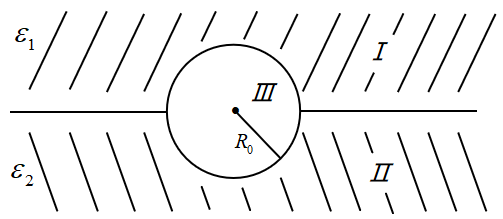
\includegraphics[height=3cm]{test/2006/pic_5.png}
        \label{fig:2006B_1}
\end{figure}
\vspace{0.4cm}

\noindent
四、\hspace{0.2em}（20分）在xy平面上，有一均匀带电，半径为a的圆盘，中心在原点处，面电荷密度为$\large{\boldsymbol{\sigma}}$（如图），求远处P点的电势。（精确到四极矩项）
\vspace{-0.8cm}
\begin{figure}[h!]
    \flushright
    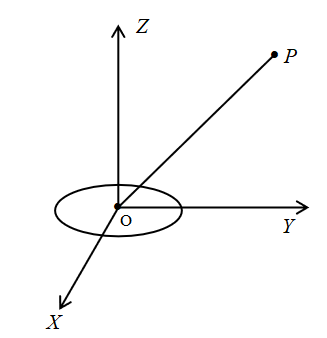
\includegraphics[height=5cm]{test/2006/pic_6.png}
        \label{fig:2006B_2}
\end{figure}

\noindent
五、\hspace{0.2em}（20分）在半径为a的圆形线圈上通有电流$I = I_0 e^{-i\omega t}$，已知$ka \ll 1 \quad (k = \frac{ \large{\boldsymbol{\omega }} }{c})$，试求:

\noindent1.\hspace{0.6em}它在r处（$r \gg \boldsymbol{\lambda}$）辐射场的电场强度和磁感应强度；

\noindent2.\hspace{0.6em}该处辐射场的能流密度；

\noindent3.\hspace{0.6em}辐射功率
\vspace{3.2cm}

\noindent
六、\hspace{0.2em}（20分）有一把直尺相对于$\large \boldsymbol{\Sigma}$坐标系静止，直尺与x轴夹角为$\large \boldsymbol{\alpha}$，今有一观测者以速度v沿x轴运动，他看到的直尺与x轴夹角$\large \boldsymbol{\alpha}^{\prime}$有何变化？
\vspace{2.4cm}


\noindent
七、\hspace{0.2em}（10分）一带电总量为Q的均匀带电球体，其半径为$\large{ {R_0}}$，距离接地的无限大导体面为a，求球内外空间任一点的电势$\large\boldsymbol{\phi}$。
\vspace{-0.6cm}
\begin{figure}[h!]
    \flushright
    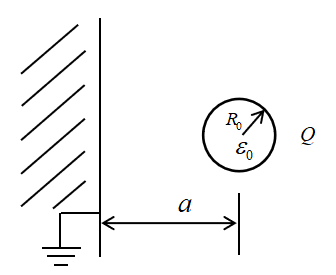
\includegraphics[height=4cm]{test/2006/pic_7.png}
        \label{fig:2006B_3}
\end{figure}

 